\documentclass[letterpaper,11pt]{article}
\usepackage[top=1.0in,bottom=1.0in,left=1.0in,right=1.0in]{geometry}
\usepackage{verbatim}
\usepackage{amssymb}
\usepackage{graphicx}
\usepackage{longtable}
\usepackage{amsfonts}
\usepackage{amsmath}
\usepackage{hyperref}
\usepackage{float}
\usepackage{setspace}
\usepackage[acronym,toc]{glossaries}  % acronyms inclusion
\usepackage{color,soul}
\makeglossary
%\newacronym{<++>}{<++>}{<++>}
\newacronym[longplural={metric tons of heavy metal}]{MTHM}{MTHM}{metric ton of heavy metal}
\newacronym{ABM}{ABM}{agent-based modeling}
\newacronym{ACDIS}{ACDIS}{Program in Arms Control \& Domestic and International Security}
\newacronym{AHTR}{AHTR}{Advanced High Temperature Reactor}
\newacronym{ANDRA}{ANDRA}{Agence Nationale pour la gestion des D\'echets RAdioactifs, the French National Agency for Radioactive Waste Management}
\newacronym{ANL}{ANL}{Argonne National Laboratory}
\newacronym{ANS}{ANS}{American Nuclear Society}
\newacronym{API}{API}{application programming interface}
\newacronym{ARE}{ARE}{Aircraft Reactor Experiment}
\newacronym{ARFC}{ARFC}{Advanced Reactors and Fuel Cycles}
\newacronym{ARMA}{ARMA}{Autoregressive Moving Average}
\newacronym{ARCH}{ARCH}{Autoregressive Heteroskedasticity}
\newacronym{ARIMA}{ARIMA}{Auto-Regressive Integrated Moving Averages}
\newacronym{ASME}{ASME}{American Society of Mechanical Engineers}
\newacronym{ATWS}{ATWS}{Anticipated Transient Without Scram}
\newacronym{BDBE}{BDBE}{Beyond Design Basis Event}
\newacronym{BIDS}{BIDS}{Berkeley Institute for Data Science}
\newacronym{BNL}{BNL}{Brookhaven National Laboratory}
\newacronym{CAFCA}{CAFCA}{ Code for Advanced Fuel Cycles Assessment }
\newacronym{CDTN}{CDTN}{Centro de Desenvolvimento da Tecnologia Nuclear}
\newacronym{CFD}{CFD}{Computational Fluid Dynamics}
\newacronym{CEA}{CEA}{Commissariat \`a l'\'Energie Atomique et aux \'Energies Alternatives}
\newacronym{CI}{CI}{continuous integration}
\newacronym{CIEMAT}{CIEMAT}{Centro de Investigaciones Energéticas, Medioambientales y Tecnológicas}
\newacronym{CNEN}{CNEN}{Comiss\~{a}o Nacional de Energia Nuclear}
\newacronym{CNERG}{CNERG}{Computational Nuclear Engineering Research Group}
\newacronym{CNRS}{CNRS}{Le Centre National De La Recherche Scientifique}
\newacronym{COSI}{COSI}{Commelini-Sicard}
\newacronym{COTS}{COTS}{commercial, off-the-shelf}
\newacronym{CSNF}{CSNF}{commercial spent nuclear fuel}
\newacronym{CTAH}{CTAHs}{Coiled Tube Air Heaters}
\newacronym{CUBIT}{CUBIT}{CUBIT Geometry and Mesh Generation Toolkit}
\newacronym{CURIE}{CURIE}{Centralized Used Fuel Resource for Information Exchange}
\newacronym{DAG}{DAG}{directed acyclic graph}
\newacronym{DANESS}{DANESS}{Dynamic Analysis of Nuclear Energy System Strategies}
\newacronym{DBE}{DBE}{Design Basis Event}
\newacronym{DEAP}{DEAP}{Distributed Evolutionary Algorithms in Python}
\newacronym{DESAE}{DESAE}{Dynamic Analysis of Nuclear Energy Systems Strategies}
\newacronym{DHS}{DHS}{Department of Homeland Security}
\newacronym{DNBR}{DNBR}{Departure from nucleate boiling ratio}
\newacronym{DOE}{DOE}{Department of Energy}
\newacronym{DRACS}{DRACS}{Direct Reactor Auxiliary Cooling System}
\newacronym{DRE}{DRE}{dynamic resource exchange}
\newacronym{DSNF}{DSNF}{DOE spent nuclear fuel}
\newacronym{DYMOND}{DYMOND}{Dynamic Model of Nuclear Development }
\newacronym{EBM}{EBM}{electron beam melting}
\newacronym{EBS}{EBS}{Engineered Barrier System}
\newacronym{EDF}{EDF}{Électricité de France}
\newacronym{EDZ}{EDZ}{Excavation Disturbed Zone}
\newacronym{EG}{EG}{Evaluation Group}
\newacronym{EIA}{EIA}{U.S. Energy Information Administration}
\newacronym{EPA}{EPA}{Environmental Protection Agency}
\newacronym{EPR}{EPR}{European Pressurized Reactors}
\newacronym{EP}{EP}{Engineering Physics}
\newacronym{EU}{EU}{European Union}
\newacronym{FCO}{FCO}{Fuel Cycle Options}
\newacronym{FCT}{FCT}{Fuel Cycle Technology}
\newacronym{FEHM}{FEHM}{Finite Element Heat and Mass Transfer}
\newacronym{FEPs}{FEPs}{Features, Events, and Processes}
\newacronym{FHR}{FHR}{Fluoride-Salt-Cooled High-Temperature Reactor}
\newacronym{FLiBe}{FLiBe}{Fluoride-Lithium-Beryllium}
\newacronym{FP}{FP}{Fission Product}
\newacronym{GDSE}{GDSE}{Generic Disposal System Environment}
\newacronym{GDSM}{GDSM}{Generic Disposal System Model}
\newacronym{GENIUSv1}{GENIUSv1}{Global Evaluation of Nuclear Infrastructure Utilization Scenarios, Version 1}
\newacronym{GENIUSv2}{GENIUSv2}{Global Evaluation of Nuclear Infrastructure Utilization Scenarios, Version 2}
\newacronym{GENIUS}{GENIUS}{Global Evaluation of Nuclear Infrastructure Utilization Scenarios}
\newacronym{GHG}{GHG}{Greenhouse Gas}
\newacronym{GPAM}{GPAM}{Generic Performance Assessment Model}
\newacronym{GRSAC}{GRSAC}{Graphite Reactor Severe Accident Code}
\newacronym{GUI}{GUI}{graphical user interface}
\newacronym{HLW}{HLW}{high level waste}
\newacronym{HPC}{HPC}{high-performance computing}
\newacronym{HTC}{HTC}{high-throughput computing}
\newacronym{HTGR}{HTGR}{High Temperature Gas-Cooled Reactor}
\newacronym{IAEA}{IAEA}{International Atomic Energy Agency}
\newacronym{IEMA}{IEMA}{Illinois Emergency Mangament Agency}
\newacronym{IHLRWM}{IHLRWM}{International High Level Radioactive Waste Management}
\newacronym{INL}{INL}{Idaho National Laboratory}
\newacronym{IPRR1}{IRP-R1}{Instituto de Pesquisas Radioativas Reator 1}
\newacronym{IRP}{IRP}{Integrated Research Project}
\newacronym{IRSN}{IRSN}{Institute for Radiological Protection and Nuclear Safety}
\newacronym{ISFSI}{ISFSI}{Independent Spent Fuel Storage Installation}
\newacronym{ISRG}{ISRG}{Independent Student Research Group}
\newacronym{JAEA}{JAEA}{Japanese Atomic Energy Agency}
\newacronym{JFNK}{JFNK}{Jacobian-Free Newton Krylov}
\newacronym{LANL}{LANL}{Los Alamos National Laboratory}
\newacronym{LBNL}{LBNL}{Lawrence Berkeley National Laboratory}
\newacronym{LCOE}{LCOE}{levelized cost of electricity}
\newacronym{L-DED}{L-DED}{laser directed energy deposition}
\newacronym{LDRD}{LDRD}{laboratory directed research and development}
\newacronym{LFR}{LFR}{Lead-Cooled Fast Reactor}
\newacronym{LLNL}{LLNL}{Lawrence Livermore National Laboratory}
\newacronym{LMFBR}{LMFBR}{Liquid Metal Fast Breeder Reactor}
\newacronym{LOFC}{LOFC}{Loss of Forced Cooling}
\newacronym{LOHS}{LOHS}{Loss of Heat Sink}
\newacronym{LOLA}{LOLA}{Loss of Large Area}
\newacronym{LP}{LP}{linear program}
\newacronym{LPD}{LPD}{Local power density}
\newacronym{LWR}{LWR}{Light Water Reactor}
\newacronym{MAGNOX}{MAGNOX}{Magnesium Alloy Graphie Moderated Gas Cooled Uranium Oxide Reactor}
\newacronym{MA}{MA}{minor actinide}
\newacronym{MCNP}{MCNP}{Monte Carlo N-Particle code}
\newacronym{MILP}{MILP}{mixed-integer linear program}
\newacronym{MIT}{MIT}{Massachusetts Institute of Technology}
\newacronym{MOAB}{MOAB}{Mesh-Oriented datABase}
\newacronym{MOOSE}{MOOSE}{Multiphysics Object-Oriented Simulation Environment}
\newacronym{MOSART}{MOSART}{Molten Salt Actinide Recycler and Transmuter}
\newacronym{MOX}{MOX}{mixed oxide}
\newacronym{MPI}{MPI}{Message Passing Interface}
\newacronym{MSBR}{MSBR}{Molten Salt Breeder Reactor}
\newacronym{MSFR}{MSFR}{Molten Salt Fast Reactor}
\newacronym{MSRE}{MSRE}{Molten Salt Reactor Experiment}
\newacronym{MSR}{MSR}{Molten Salt Reactor}
\newacronym{NAGRA}{NAGRA}{National Cooperative for the Disposal of Radioactive Waste}
\newacronym{NEAMS}{NEAMS}{Nuclear Engineering Advanced Modeling and Simulation}
\newacronym{NEUP}{NEUP}{Nuclear Energy University Programs}
\newacronym{NFC}{NFC}{Nuclear Fuel Cycle}
\newacronym{NFCSim}{NFCSim}{Nuclear Fuel Cycle Simulator}
\newacronym{NGNP}{NGNP}{Next Generation Nuclear Plant}
\newacronym{NMWPC}{NMWPC}{Nuclear MW Per Capita}
\newacronym{NNL}{NNL}{National Nuclear Laboratory}
\newacronym{NNSA}{NNSA}{National Nuclear Security Administration}
\newacronym{NPP}{NPP}{Nuclear Power Plant}
\newacronym{NPRE}{NPRE}{Department of Nuclear, Plasma, and Radiological Engineering}
\newacronym{NQA1}{NQA-1}{Nuclear Quality Assurance - 1}
\newacronym{NRC}{NRC}{Nuclear Regulatory Commission}
\newacronym{NSF}{NSF}{National Science Foundation}
\newacronym{NSSC}{NSSC}{Nuclear Science and Security Consortium}
\newacronym{NUWASTE}{NUWASTE}{Nuclear Waste Assessment System for Technical Evaluation}
\newacronym{NWF}{NWF}{Nuclear Waste Fund}
\newacronym{NWTRB}{NWTRB}{Nuclear Waste Technical Review Board}
\newacronym{OCRWM}{OCRWM}{Office of Civilian Radioactive Waste Management}
\newacronym{OECD}{OECD}{Organisation for Economic Co-operation and Development}
\newacronym{ORION}{ORION}{ORION}
\newacronym{ORNL}{ORNL}{Oak Ridge National Laboratory}
\newacronym{PARCS}{PARCS}{Purdue Advanced Reactor Core Simulator}
\newacronym{PBAHTR}{PB-AHTR}{Pebble Bed Advanced High Temperature Reactor}
\newacronym{PBFHR}{PB-FHR}{Pebble-Bed Fluoride-Salt-Cooled High-Temperature Reactor}
\newacronym{PEI}{PEI}{Peak Environmental Impact}
\newacronym{PH}{PRONGHORN}{PRONGHORN}
\newacronym{PPF}{PPF}{Power peaking factor}
\newacronym{PRIS}{PRIS}{Power Reactor Information System}
\newacronym{PRKE}{PRKE}{Point Reactor Kinetics Equations}
\newacronym{PSPG}{PSPG}{Pressure-Stabilizing/Petrov-Galerkin}
\newacronym{PWAR}{PWAR}{Pratt and Whitney Aircraft Reactor}
\newacronym{PWR}{PWR}{Pressurized Water Reactor}
\newacronym{PyNE}{PyNE}{Python toolkit for Nuclear Engineering}
\newacronym{PyRK}{PyRK}{Python for Reactor Kinetics}
\newacronym{QA}{QA}{quality assurance}
\newacronym{RDD}{RD\&D}{Research Development and Demonstration}
\newacronym{RD}{R\&D}{Research and Development}
\newacronym{REE}{REE}{rare earth element}
\newacronym{RELAP}{RELAP}{Reactor Excursion and Leak Analysis Program}
\newacronym{RIA}{RIA}{Reactivity Insertion Accident}
\newacronym{RIF}{RIF}{Region-Institution-Facility}
\newacronym{SA}{SA}{Sensitivity Analysis}
\newacronym{SCK CEN}{SCK CEN}{Studiecentrum voor Kernenergie}
\newacronym{SFR}{SFR}{Sodium-Cooled Fast Reactor}
\newacronym{SINDAG}{SINDA{\textbackslash}G}{Systems Improved Numerical Differencing Analyzer $\backslash$ Gaski}
\newacronym{SKB}{SKB}{Svensk K\"{a}rnbr\"{a}nslehantering AB}
\newacronym{SNF}{SNF}{spent nuclear fuel}
\newacronym{SNL}{SNL}{Sandia National Laboratory}
\newacronym{SLM}{SLM}{selective laser melting}
\newacronym{STC}{STC}{specific temperature change}
\newacronym{SUPG}{SUPG}{Streamline-Upwind/Petrov-Galerkin}
\newacronym{SWF}{SWF}{Separations and Waste Forms}
\newacronym{SWU}{SWU}{Separative Work Unit}
\newacronym{TRIGA}{TRIGA}{Training Research Isotope General Atomic}
\newacronym{TRISO}{TRISO}{Tristructural Isotropic}
\newacronym{TSM}{TSM}{Total System Model}
\newacronym{TSPA}{TSPA}{Total System Performance Assessment for the Yucca Mountain License Application}
\newacronym{ThOX}{ThOX}{thorium oxide}
\newacronym{UFD}{UFD}{Used Fuel Disposition}
\newacronym{UML}{UML}{Unified Modeling Language}
\newacronym{UOX}{UOX}{uranium oxide}
\newacronym{UQ}{UQ}{uncertainty quantification}
\newacronym{US}{US}{United States}
\newacronym{USC}{USC}{University of South Carolina}
\newacronym{UIUC}{UIUC}{University of Illinois at Urbana-Champaign}
\newacronym{UT Austin}{UT Austin}{The University of Texas at Austin}
\newacronym{UW}{UW}{University of Wisconsin}
\newacronym{VISION}{VISION}{the Verifiable Fuel Cycle Simulation Model}
\newacronym{VVER}{VVER}{Voda-Vodyanoi Energetichesky Reaktor (Russian Pressurized Water Reactor)}
\newacronym{VV}{V\&V}{verification and validation}
\newacronym{YMR}{YMR}{Yucca Mountain Repository Site}


\usepackage{tikz}
\usetikzlibrary{positioning, arrows, decorations, shapes}
\usetikzlibrary{shapes.geometric,arrows}

\definecolor{illiniblue}{HTML}{B1C6E2}
\definecolor{illiniorange}{HTML}{f8c2a2}
\definecolor{pink}{HTML}{e2b1c2}
\definecolor{green}{HTML}{c2e2b1}
\definecolor{purple}{HTML}{b9b1e2}
\tikzstyle{snoblock} = [rectangle, 
text width=5em, text centered,  minimum height=0em]
\tikzstyle{noblock} = [rectangle, 
text width=5em, text centered,  minimum height=3em]
\tikzstyle{loblock} = [rectangle, draw, fill=illiniorange, 
text width=15em, text centered, rounded corners, minimum height=3em]
\tikzstyle{lbblock} = [rectangle, draw, fill=illiniblue, 
text width=15em, text centered, rounded corners, minimum height=3em]
\tikzstyle{oblock} = [rectangle, draw, fill=illiniorange, 
text width=10em, text centered, rounded corners, minimum height=3em]
\tikzstyle{bblock} = [rectangle, draw, fill=illiniblue, 
text width=10em, text centered, rounded corners, minimum height=3em]
\tikzstyle{arrow} = [thick,->,>=stealth]
\tikzstyle{pblock} = [rectangle, draw, fill=pink, 
text width=10em, text centered, rounded corners, minimum height=3em]
\tikzstyle{gblock} = [rectangle, draw, fill=green, 
text width=10em, text centered, rounded corners, minimum height=3em]
\tikzstyle{ppblock} = [rectangle, draw, fill=purple, 
text width=10em, text centered, rounded corners, minimum height=3em]
\tikzstyle{lppblock} = [rectangle, draw, fill=purple, 
text width=15em, text centered, rounded corners, minimum height=3em]
\tikzstyle{arrow} = [thick,->,>=stealth]
\tikzstyle{bbblock} = [rectangle, draw, fill=illiniblue, 
text width=1em, text centered, rounded corners, minimum height=1em]
\tikzstyle{boblock} = [rectangle, draw, fill=illiniorange, 
text width=1em, text centered, rounded corners, minimum height=1em]
\tikzstyle{bpblock} = [rectangle, draw, fill=pink, 
text width=1em, text centered, rounded corners, minimum height=1em]
\tikzstyle{bgblock} = [rectangle, draw, fill=green, 
text width=1em, text centered, rounded corners, minimum height=1em]
\tikzstyle{bppblock} = [rectangle, draw, fill=purple, 
text width=1em, text centered, rounded corners, minimum height=1em]

\author{Gwendolyn J. Chee}

\title{Generative Reactor Design}
\begin{document}
\maketitle
\hrulefill
\onehalfspacing

\section{Generative Design}
% What is generative design? How does it work? 
Generative design is an exploratory design method that autonomously 
generates optimal designs by iteratively varying design geometry 
to meet user-defined performance metrics 
\cite{krish_practical_2011,oh_deep_2019}.
The user defines the design parameters and the generative 
design software helps the user create many solutions 
simultaneously \cite{autodesk_autodesk_2020}. 
This sometimes results in unanticipated unique solutions, that 
would have been difficult to discover using traditional methods
\cite{autodesk_autodesk_2020}.
Generative design varies the parameters of the problem definition
\cite{matejka_dream_2018}. 
At each iteration step, the design is evaluated on the 
performance metrics. 
Based on the results, the generative design algorithm changes the 
interval allowed for each design geometry variable, refining 
design constraints (problem definition) and moving towards 
designs that best meets performance metrics.

There is confusion to how generative design differs from other shape 
optimization tools. 
Generative design is more than topology optimization which has been 
around since 1988 \cite{bendsoe_generating_1988}. 
Topology optimization requires the user to start with a complete design 
and the software improves it by removing material, it answers the 
fundamental engineering question of how to place material in a domain space 
to obtain best structural performance \cite{sigmund_topology_2013}.   
Generative design does not require the user to start with a complete design, but 
instead a few design constraints. 
Table \ref{tab:compare} summarizes the differences between generative design and 
traditional design optimization tools. 

\begin{table}[!htbp]
        \caption{Comparison of generative design and traditional design optimization tools
        \cite{autodesk_fusion_2020}.}
        \label{tab:compare}
        \centering
        \doublespacing
        \small
        \begin{tabular}{p{3.7cm}|p{5.5cm}p{6cm}}
        \hline
        \textbf{Point of Comparison} & \textbf{Generative Design} & \textbf{Traditional Design Optimization Tools}  \\ \hline
        Initial input & A few design constraints & Complete design \\ 
        No. of outcomes & Generates a wide set of designs that meets design constraints & Identifies one unique design that meets constraints \\   
        Solving strategies & Uses multiple strategies to solve design problem & Mainly uses topology optimization solutions \\ \hline
        \end{tabular}
\end{table}

% How does it actually work? What models? 

\subsection{State of Work}
Generative design is used in the following industries: 
automotive \cite{deplazes_autodesk_2019}, aerospace \cite{byrne_evolving_2014},
architecture, civil engineering, construction, product design etc. 
For the automotive and aerospace industries, the goal of generative 
design is to decrease 
the weight of the vehicle while ensuring each part can continue to 
withstand the stresses and strains that are put on it within a 
safety factor. 
These industries can rely on commerical softwares such as 
Autodesk Fusion360 \cite{autodesk_autodesk_2020} and  
SolidWorks Topology \cite{lombard_solidworks_2008}
to produce their generative designs, since these softwares have 
structural simulation-based generative design technology.  

Civil engineering and architecture generative design projects use specific s

\subsection{Optimization Techniques}
Multi-objective design problems inevitably require a trade off between 
desirable attributes \cite{byrne_evolving_2014,simon_sciences_2019}. 
In nuclear reactor design there are many trade offs, one example is the 
trade-off between neutron economy and fuel enrichment. 
A reactor design must have sufficient neutron economy to ensure criticality, 
but must also have a low fuel enrichment to reduce proliferation risk.
Conflicting objectives means that there is no one perfect solution, but a set
of equally optimal solutions \cite{byrne_evolving_2014}.
Multi-objective problems are difficult to optimize, such problems 
cannot be handled by classical optimization methods such as gradient 
methods, because they tend to only find the local optimum 
\cite{renner_genetic_2003} and are efficient for a narrow subset 
of problems \cite{zames_genetic_1981}. 

Evolutionary algorithms have proven to be successful 
methods to optimize multi-objective problems \cite{krish_practical_2011} as 
they can find a solution near the global optimum \cite{renner_genetic_2003}. 
The most popular evolutionary algorithms used to solve multi-objective 
problems are genetic algorithms 
\cite{byrne_evolving_2014, krish_practical_2011}. 
Genetic algorithms differ from classical optimization techniques in four ways 
\cite{zames_genetic_1981}: 
\begin{enumerate}
        \item Work with each parameter's constraints, not
        the parameters themselves. 
        \item Search a population of points, not a single point. 
        \item Use a user-defined objective function in the 
        optimization process, not derivatives or other auxillary knowledge. 
        \item Use stochastic rules, not deterministic rules. 
\end{enumerate}

\subsubsection{Genetic Algorithms}
Genetic algorithms imitate natural selection to evolve solutions 
by (1) maintaining a population of solutions, (2) allowing 
fitter solutions reproduce, and (3) letting lesser fit solutions die off, 
resulting in final solutions that are better than the previous generations 
\cite{renner_genetic_2003}. 
Figure \ref{fig:genetic_alg} depicts the iterative process of using a genetic 
algorithm to solve a problem. 
The key part of this process is defining evaluation and termination criteria. 
Evaluation criteria refers to the performance metrics that each solution is 
measured against. 
Termination criteria refers to the range of values for each performance metric
that a solution must meet to be considered `good enough'. 
Attainment of optimum is much less important for complex systems, the goal is 
to get a good solution without sacrificing the level of performance (speed of 
code) \cite{zames_genetic_1981}. 

\begin{figure}[!htbp]
        \centering
        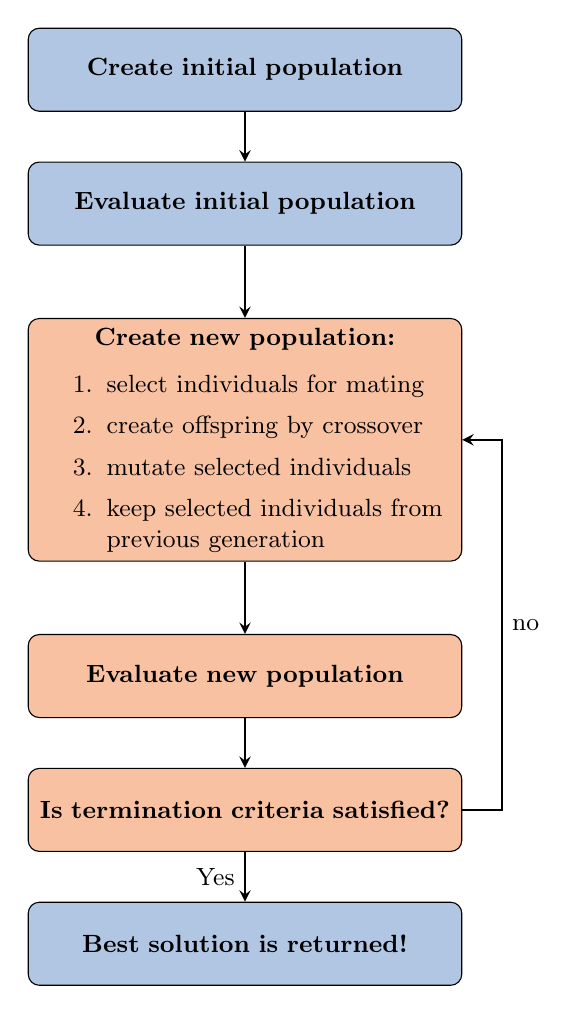
\begin{tikzpicture}[node distance=1.7cm]
                \tikzstyle{every node}=[font=\small]
                \node (1) [lbblock] {\textbf{Create initial population}};
                \node (2) [lbblock, below of=1] {\textbf{Evaluate initial population}};
                \node (3) [loblock, below of=2, yshift = -1.3cm] {\textbf{Create new population:} \\ 
                \begin{enumerate} \item select individuals for mating 
                                  \item create offspring by crossover 
                                  \item mutate selected individuals 
                                  \item keep selected individuals from previous generation
                                 \end{enumerate}};
                \node (4) [loblock, below of=3, yshift=-1.3cm] {\textbf{Evaluate new population}};
                \node (5) [loblock, below of=4] {\textbf{Is termination criteria satisfied?}};
                \node (6) [lbblock, below of=5] {\textbf{Best solution is returned!}};
                \draw [arrow] (1) -- (2);
                \draw [arrow] (2) -- (3);
                \draw [arrow] (3) -- (4);
                \draw [arrow] (4) -- (5);
                \draw [arrow] (5) -- node[anchor=east] {Yes} (6);
                \draw [arrow] (5) -- ([shift={(0.5cm,0cm)}]5.east)-- node[anchor=west] {no} ([shift={(0.5cm,0cm)}]3.east)--(3);
        \end{tikzpicture}
        \caption{Process of solving a problem with genetic algorithm 
        \cite{renner_genetic_2003}. When a population does not meet termination 
        criteria, a new generation is created. This occurs iteratively till the 
        termination criteria is met. }
        \label{fig:genetic_alg}
\end{figure}

Two types of genetic algorithms are typically used to solve shape 
optimization problems: parametric and cell. 
Parametric genetic algorithms optimize complex shapes by varying parametric variables
to meet the desired design performance \cite{von_buelow_paragen_2012}.
Examples of parametric variables are: diameter of a sphere, twist angle of a cylinder, 
etc.  
Optimization of aerodynamic configurations \cite{makinen_multidisciplinary_1999}, 
and truss and bridge structures \cite{raich_evolving_2000} used parametric 
genetic algorithms.
Cell genetic algorithms represent the shape of an object to be optimized in 
small subdivided rectangular domains (pixels in 2D, voxels in 3D) 
\cite{renner_genetic_2003}. 
Figure \ref{fig:cell} shows an example of cell representation. 
Cell genetic algorithms are advantageous compared to parametric genetic 
algorithms since the initial structure and topology of the object need not 
be created and is instead developed through the iterative optimization 
process \cite{renner_genetic_2003}. 
Both parametric and cell genetic algorithms will be explored for the generative 
reactor design problem. 

\begin{figure}[!htbp]
	\begin{center}
		\includegraphics[scale=0.25]{./figures/cell.png}
        \end{center}	
        \caption{Cell representation in 2D \cite{renner_genetic_2003}.}
        \label{fig:cell}
\end{figure}
\section{Generative Reactor Design}
For nuclear reactors, generative design is constrained by 
variables such as mass or volume of fuel, fuel enrichment, effectiveness 
of heat transfer, effective neutron multiplication factor, etc. 
Nuclear reactors not only experience physical forces, but also
require evaluation of the neutronics of the system, therefore generative design of 
a nuclear reactor cannot make use of tools such as Autodesk Fusion360 or SolidWorks 
Topology. 
Therefore, a framework that couples well-developed advanced genetic algorithms 
with well-supported monte-carlo particle transport 
codes (Serpent \cite{leppanen_serpent_2014}, 
MCNP \cite{werner_mcnp6._2018}, etc.) and thermal hydraulics 
codes (RELAP7 \cite{andrs_relap-7_2012} etc.)
must be created to successfully produce generative reactor designs. 

\subsection{Workflow}
% How the genetic algorithm is coupled with a CAD designer and analysis tool 
% (serpent/RELAP)
% CAD designer > grasshopper3d (see Bryne Paper)
Figure \ref{fig:workflow} depicts a framework for leveraging genetic algorithms
to design nuclear reactors. 
This is a general framework that does not specify algorithms or analytical 
softwares. 
Instead, it provides placeholders for algorithm and software types, so 
that a user may choose the types of algorithms and softwares they want to use in 
their mission towards using generative design to design a nuclear reactor. 
Table \ref{tab:examples} lists algorithm and software types that could be used 
in the framework. 

\begin{figure}[!htbp]
        \centering
        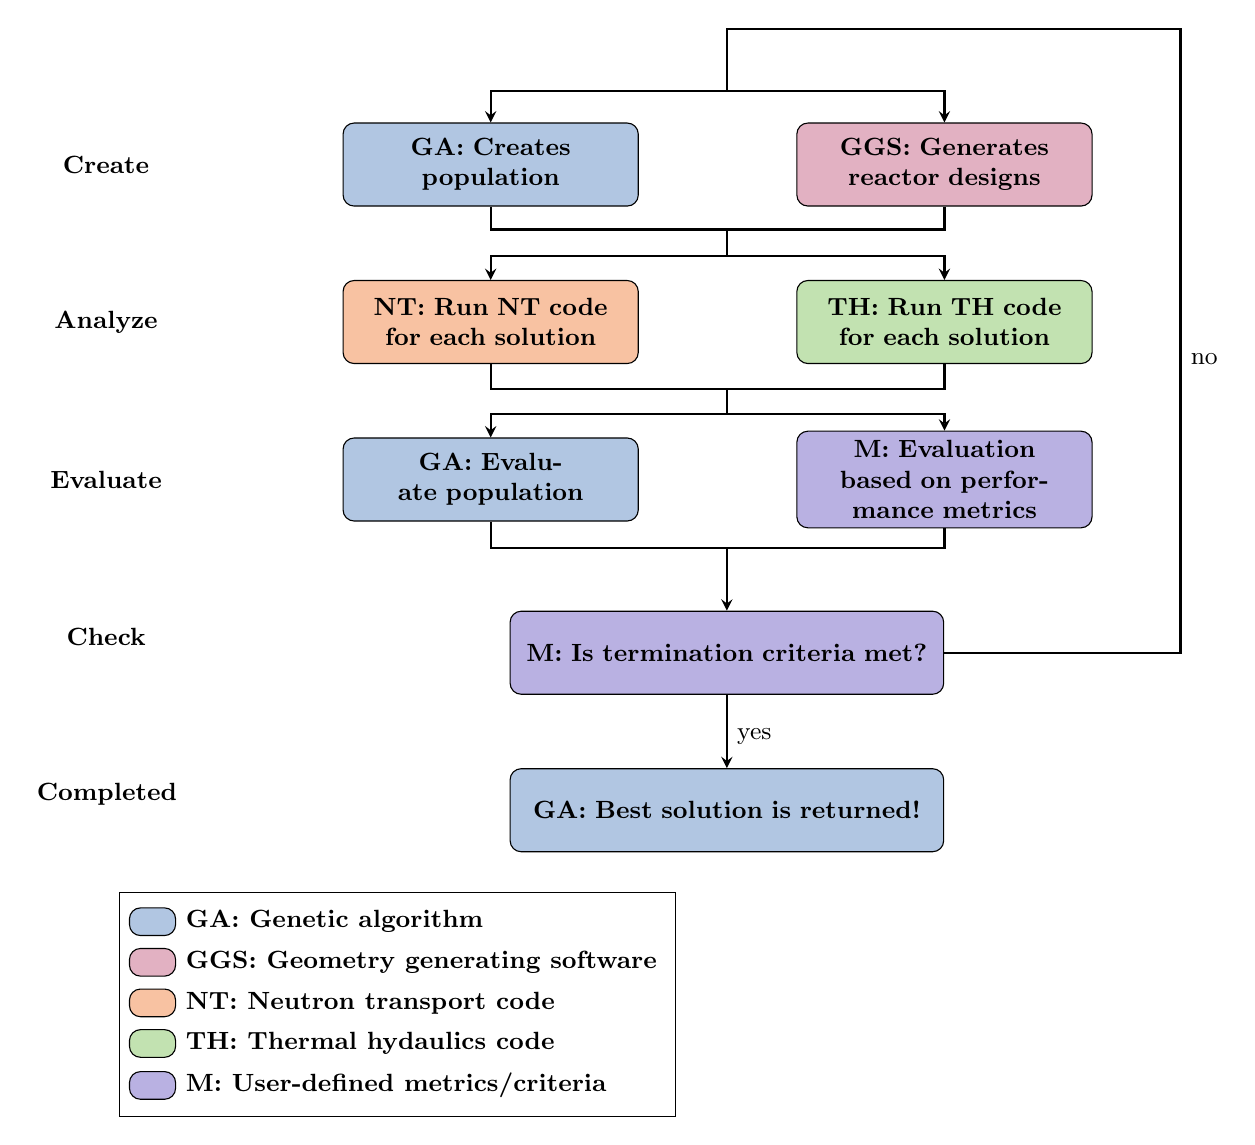
\begin{tikzpicture}[node distance=2cm]
                \tikzstyle{every node}=[font=\small]
                \node[anchor=west] (1) [noblock] {\textbf{Create}};
                \node (2) [bblock, right=of 1] {\textbf{GA: Creates population}};
                \node (3) [pblock, right=of 2] {\textbf{GGS: Generates reactor designs}};
                \node[anchor=west] (4) [noblock, below of= 1] {\textbf{Analyze}};
                \node (5) [oblock, below of =2]{\textbf{NT: Run NT code for each solution}};
                \node (6) [gblock, right=of 5]{\textbf{TH: Run TH code for each solution}};
                \node[anchor=west] (7) [noblock, below of= 4] {\textbf{Evaluate}};
                \node (8) [bblock, below of =5] {\textbf{GA: Evaluate population}};
                \node (9) [ppblock, right=of 8] {\textbf{M: Evaluation based on performance metrics}};
                \node[anchor=west] (10) [noblock, below of= 7] {\textbf{Check}};
                \node (11) [lppblock, below of=8, xshift=3cm, yshift=-0.2cm] {\textbf{M: Is termination criteria met?}};
                \node (16) [lbblock, below of = 11] {\textbf{GA: Best solution is returned!}};
                \node[anchor=west] (12) [snoblock, above of= 2, xshift=3cm, yshift=-1.1cm] {};
                \node[anchor=west] (13) [snoblock, below of=12,yshift=-0.15cm] {};
                \node[anchor=west] (14) [snoblock, below of=13,yshift=-0.02cm] {};
                \node[anchor=west] (15) [snoblock, below of=14,yshift=-0.02cm] {};
                \node[anchor=west] (17) [noblock, below of= 10] {\textbf{Completed}};
                \draw [-,thick] (11) -- ([shift={(3cm,0cm)}]11.east) |- node[anchor=west, yshift=-4.2cm] {no} ([shift={(0cm,0.7cm)}]12.north)--(12);
                \draw [arrow] (12) -- ([shift={(0cm,0cm)}]12.north) |- ([shift={(0cm,0.4cm)}]2.north)--(2);
                \draw [arrow] (12) -- ([shift={(0cm,0cm)}]12.north) |- ([shift={(0cm,0.4cm)}]3.north)--(3);
                \draw [-,thick] (2) -- ([shift={(0cm,0cm)}]2.south) |- ([shift={(0cm,0.3cm)}]13.north)--(13);
                \draw [-,thick] (3) -- ([shift={(0cm,0cm)}]3.south) |- ([shift={(0cm,0.3cm)}]13.north)--(13);
                \draw [arrow] (13) -- ([shift={(0cm,0cm)}]13.north) |- ([shift={(0cm,0.3cm)}]5.north)--(5);
                \draw [arrow] (13) -- ([shift={(0cm,0cm)}]13.north) |- ([shift={(0cm,0.3cm)}]6.north)--(6);
                \draw [-,thick] (5) -- ([shift={(0cm,0cm)}]5.south) |- ([shift={(0cm,0.3cm)}]14.north)--(14);
                \draw [-,thick] (6) -- ([shift={(0cm,0cm)}]6.south) |- ([shift={(0cm,0.3cm)}]14.north)--(14);
                \draw [arrow] (14) -- ([shift={(0cm,0cm)}]14.north) |- ([shift={(0cm,0.3cm)}]8.north)--(8);
                \draw [arrow] (14) -- ([shift={(0cm,0cm)}]14.north) |- ([shift={(0cm,0.21cm)}]9.north)--(9);
                \draw [-,thick] (8) -- ([shift={(0cm,0cm)}]8.south) |- ([shift={(0cm,0.3cm)}]15.north)--(15);
                \draw [-,thick] (9) -- ([shift={(0cm,0cm)}]9.south) |- ([shift={(0cm,0.3cm)}]15.north)--(15);
                \draw [arrow] (15) -- ([shift={(0cm,0cm)}]15.north) |- ([shift={(0cm,0.1cm)}]11.north)--(11);
                \draw [arrow] (11) -- ([shift={(0cm,0cm)}]11.south) |- node[anchor=west, yshift=0.3cm] {yes} ([shift={(0cm,0.1cm)}]16.north)--(16);
                \matrix [draw,below left,yshift=-0.5cm, xshift=-7cm] at (current bounding box.south east) {
                \node [bbblock,label=right:\textbf{GA: Genetic algorithm}] {}; \\
                \node [bpblock,label=right:\textbf{GGS: Geometry generating software}] {}; \\
                \node [boblock,label=right:\textbf{NT: Neutron transport code}] {}; \\
                \node [bgblock,label=right:\textbf{TH: Thermal hydaulics code}] {}; \\
                \node [bppblock,label=right:\textbf{M: User-defined metrics/criteria}] {}; \\
                };
        \end{tikzpicture}
        \caption{Generative reactor design framework. Each component of the 
        framework is user-selected.}
        \label{fig:workflow}
\end{figure}

\begin{table}[!htbp]
        \caption{Example algorithm and software types to populate generative reactor 
        design framework (Fig \ref{fig:workflow}).}
        \label{tab:examples}
        \centering
        \doublespacing
        \small
        \begin{tabular}{lp{10cm}}
        \hline
        \textbf{Framework Component} & \textbf{Examples}\\ \hline
        Genetic algorithm driver & DEAP \cite{fortin_deap_2012} \\
        Geometry generating software & Trelis \cite{noauthor_trelis_2018}, FreeCAD \cite{falck_freecad_2012}, SolidWorks \cite{lombard_solidworks_2008}, grasshopper3d \cite{rutten_grasshopper3d_2015}, GenerativeComponents \cite{aish_bentleys_2003}, Trilinos \cite{heroux_overview_2003} \\
        Neutron transport code & Serpent \cite{leppanen_serpent_2014}, MCNP \cite{werner_mcnp6._2018}, SCALE \cite{bucholz_scale:_1982}, OpenMC \cite{romano_openmc_2013} \\ 
        Thermal hydraulics code & RELAP5-3D \cite{strydom_comparison_2016}, RELAP7 \cite{andrs_relap-7_2012}, TRACE \cite{xu_multi-physics_2006}\\
        User-defined metrics/criteria & keff, heat transfer rate, fuel enrichment, mass of fuel \\ \hline
\end{tabular}
\end{table}

\subsection{Software}
The generative reactor design framework proposed (Fig. \ref{fig:workflow}) 
has many coupled components. 
To minimize the amount of coupling required, software is chosen with 
framework-leanness in mind. 
The shortlisted software will be evaluated based on the clearly 
defined requirements of each component. 
Each iteration of the framework requires the neutron transport code, 
the thermal hydraulics code, and evaluation to be run for each 
nuclear reactor geometry (individual) generated by the genetic algorithm. 
Therefore, to ensure efficiency of the framework, the individual runs 
must be parallelized. 
The generative reactor design framework is computation-heavy. 
To produce results in a timely manner, a high performance computer 
such as Blue Waters \cite{ncsa_about_2017} will be used. 
In summary, each component's software is chosen based on these 
conditions: 
\begin{enumerate}
    \item It best meets the clearly defined requirements 
    its respective component. 
    \item It is parallelizable. 
    \item It is compatible with a high performance computer. 
    \item It is open-source and free (preferable but not required). 
\end{enumerate}

The subsequent subsections will define the requirements of each 
component in the generative reactor framework, the software considered, 
and an explanation justifying the final software choice. 

\subsubsection{Genetic Algorithm Driver}
Evolutionary algorithm computation is a sophisticated field with diverse
techniques and mechanisms, resulting in even well designed frameworks 
being complicated under the hood \cite{fortin_deap_2012}. 
These implementation intricacies are difficult to extend since it requires 
the user to edit the source code. 
This is concerning since using evolutionary algorithms to solve unique 
real-world problems requires customization of algorithms 
\cite{fortin_deap_2012}. 
Therefore, an evolutionary algorithm computation framework that gives 
the user the capability to build custom evolutionary algorithms is 
required for this project. 

There are many evolutionary algorithm computation packages 
available: \gls{DEAP} \cite{fortin_deap_2012}, 
inspyred \cite{garrett_inspyred_2014}, 
Pyevolve \cite{perone_pyevolve_2009}, and
OpenBEAGLE \cite{gagne_open_2002}. 
DEAP is the most newly created package and places a high value on 
code compactness and code clarity \cite{fortin_deap_2012}. 
A comparison of the number of lines of code each package requires 
to define different components of a test problem, and \gls{DEAP} 
was the only framework that completely defined the test problem 
in less than one hundred lines of code \cite{fortin_deap_2012}.
\gls{DEAP} is the only framework that allows the user to rapidly 
prototype evolutionary algorithms and define custom algorithms without 
having to dig deep into the source code to modify lines, making it 
the code of choice for the genetic algorithm driver component of 
the generative reactor design framework. 

\subsubsection{Geometry Generating Software}


\subsubsection{Neutron Transport Code}

\subsubsection{Thermal Hydraulics Code}

\subsection{Evaluation Metrics}


\section{Reactor}
For this project, generative reactor design is explored for the 
\gls{FHR}. 
% Why it was chosen 
% What is it? 
% Benchmark? 
\section{Method}

\subsection{Genetic Algorithm}

\subsection{Reactor Geometry Generation}
The biggest challenge for generatively designing reactor geometries with 
non-classical shapes is defining the parameters to be varied. 
A good balance must be struck between number of degrees of freedom (parameters) 
and giving the algorithm the flexibility to create unique geometries. 
Bergmann et al \cite{bergmann_simulation_2018} described a 2D re-entrant hole 
in the Swiss Spallation Neutron Source with 9 variables that allowed the genetic 
algorithm to cover a large exploration space of CAD geometries. 
The 9 variables included five distance values and four angle values. 
Veenstra et all \cite{veenstra_evolution_2018} described the undulation of 
a Knife-fish soft robot with a fourier series. 
The genetic algorithm varied five terms in the fourier series to find the undulation 
that resulted in the fastest swimming. 

For this project, we can learn from them by creating parameters that
express reactor geometry simply while allowing for a large exploration space. 

\subsubsection{Constraints}
Reactor geometry constraints must be defined to ensure that only realistic 
geometries are accepted. 
Constraints are: 
\begin{itemize}
    \item Each cooling channel must fully go through the reactor from top to 
    bottom. This is to prevent cooling channels from not having a through 
    path, resulting in lack of heat transfer. 
\end{itemize}

\subsubsection{Parameters}



\pagebreak
\bibliographystyle{plain}
\bibliography{2020-generative-reactor-design-lit-review}
\end{document}

